\chapter{Quantification of incomparability for pairs of states} \label{chap:incomparability} \label{chap:criteria}

This chapter first shows an improvement over traditional entropic separability criteria that can be achieved using the lattice. As this improvement depends on the incomparability between the two reduced states'eigenvalues, this chapter then tries to quantify the amount of incomparability between probability vectors by defining new objects . It is interesting to note that some unpublished work attempting to quantify the incomparability of quantum states (without the lattice) does exist in Ref. \cite{hu_characterizing_2018}, however the proposed measures do not seem very natural.



\section{Motivation} \label{sec:incomparability_motivation}

\subsection{Improved separability criterion based on meet}

The second result of this master thesis is to improve some entropic criteria tied to majorization relations. As stated in theorem \ref{th:majorization_separability_criterion}, if a bipartite state $\rho^{AB}$ is separable, then

\begin{equation}
    \lambda^{AB} \prec \lambda^A \quad \text{and} \quad \lambda^{AB} \prec \lambda^{B},
\end{equation}

where $\lambda^X$ is the ordered vector of eigenvalues of the density matrix of system $X$. By Schur-concavity of $H$, this directly implies

\begin{equation}
    H(\lambda^{AB}) \geq H(\lambda^A) \quad \text{and} \quad H(\lambda^{AB}) \geq H(\lambda^B).
\end{equation}

These entropic inequalities\footnote{Historically, these entropic inequalities (expressed equivalently in von Neumann entropies) were known before the strengthening to a majorization relation \cite{cerf_negative_1997, nielsen_separable_2001}.} are of course not as strong as the majorization relations we deduced them from, as illustrated in the example from section \ref{sec:majorization_separability_criterion}. Using the lattice, however, the entropic condition can be strengthened. The relations $\lambda^{AB} \prec \lambda^A$ and $\lambda^{AB} \prec \lambda^{B}$ mean that $\lambda^{AB}$ is majorized by both $\lambda^A$ and $\lambda^B$. By definition, the meet of $\lambda^A$ and $\lambda^B$ is the vector $\lambda^A \wedge \lambda^B$ that majorizes all the vectors that are majorized by both $\lambda^A$ and $\lambda^B$. This fact can also be restated as 

\begin{equation}
    \mathcal{T}_-(\lambda^A) \cap \mathcal{T}_-(\lambda^B) = \mathcal{T}_-(\lambda^A \wedge \lambda^B),
\end{equation}

\noindent using definition \ref{def:majorization_cones} of majorization cones. Applying this to the separability criterion, we get that if $\rho^{AB}$ is a separable state, then

\begin{equation}
    \lambda^{AB} \prec \lambda^A \; \text{and} \; \lambda^{AB} \prec \lambda^{B} \; \iff \; \lambda^{AB} \prec \lambda^A \wedge \lambda^B \; \implies \; H(\lambda^{AB}) \geq H(\lambda^A \wedge \lambda^B).
\end{equation}

This new formulation in terms of entropies is a strengthening of the initial entropic criterion, providing a better lower bound on the entropy of a separable state. However, it is still not as strong as the majorization criterion itself. Moreover, this new entropic criterion based on the meet is not very interesting for pure bipartite states because of Corollary \ref{cor:reduced_schmidt}, which essentially states that $\lambda^A = \lambda^B$ if $\rho^{AB}$ is pure. In that case $\lambda^A \wedge \lambda^B = \lambda^A = \lambda^B$, and the new entropic criterion reduces to the original one. While pure bipartite states are the more interesting states for quantum computation, as decoherence (i.e. losing purity by interacting with the environment) is never a desired feature for qubits as mixed states introduce uncertainty into computations, in practice noise always makes states at least slightly mixed. Figure \ref{fig:improved_criterion} illustrates the new criterion.

\begin{figure}[h!]
    \centering
    \begin{tikzpicture}[scale=0.9]
        % draw cone of p
        \coordinate (A) at (-2, 3);
        \coordinate (B) at (1, -1.5);
        \draw[dotted] [name path=A--B, color=gray] (A) -- (B);
        \coordinate (C) at (-1,-1.5);
        \coordinate (D) at (2,3);
        \draw[dotted] [name path=C--D, color=gray] (C) -- (D);
        \path [name intersections={of=A--B and C--D,by=E}];
        \node [fill=black,inner sep=1pt,label=180:$\lambda^A$] at (E) {};
        % draw cone of q
        \coordinate (F) at (-0.166,3);
        \coordinate (G) at (2.833, -1.5);
        \draw[dotted] [name path=F--G, color=gray] (F) -- (G);
        \coordinate (H) at (2.166,-1.5);
        \coordinate (I) at (4.966,3);
        \draw[dotted] [name path=H--I, color=gray] (H) -- (I);
        \path [name intersections={of=F--G and H--I,by=J}];
        \node [fill=black,inner sep=1pt,label=0:$\lambda^B$] at (J) {};
        %intersections of the 2 cones
        \path [name intersections={of=F--G and C--D,by=K}];
        %\path [name intersections={of=H--I and A--B,by=L}];
        \node [fill=black,inner sep=1pt,label=90:$\lambda^A \wedge \lambda^B$] at (K) {};
        %\node [fill=black,inner sep=1pt] at (L) {};
        %\node [inner sep=4pt, label=270:$p \vee q$] at (L) {}; % virtual point to set the label further away (otherwise the fill gets bigger too)
        % create the entropy arrow
        \coordinate (M) at (-3, -1.5);
        \coordinate (N) at (-3, 3);
        \coordinate (N') at (-3, 3.3);
        \coordinate (O) at (5, 1.33);
        \coordinate (P) at (5, 3);
        \coordinate (Q) at (5, -1.5);
        \coordinate (R) at (-3, 1.33);
        \coordinate (S) at (-3.5, 1.33);

        \draw[->] (M) -- (N');
        \node [inner sep=0pt, label=180:$H(\lambda^{AB})$] at (N') {};
        \draw[dotted] [name path=old_left, color=gray] (E) -| (M);
        \draw[dotted] [name path=old_right, color=gray] (E) -| (5,0);
        \draw[dotted] [name path=new_left, color=gray] (K) -| (S);
        \draw[dotted] [name path=new_right, color=gray] (K) -| (O);
        % fill the 2 zones for the criterion
        \fill[fill=blue, opacity=0.15] (N) -- (R) -- (O) -- (P) -- cycle;
        \fill[fill=red, opacity=0.15] (M) -- (R) -- (O) -- (Q) -- cycle;
        \node [inner sep=3pt, label=135:{Maybe entangled, maybe separable}] at (R) {};
        \node [inner sep=3pt, label=225:{Entangled}] at (R) {};

    \end{tikzpicture}
    \caption{Depiction of the improved entropic criterion for entanglement. The previous criterion could not decide whether states with $\lambda^{AB}$ with an entropy between the two horizontal doted lines going through $\lambda^A$ and $\lambda^A \wedge \lambda^B$ were entangled. The new criterion shows that they are.}
    \label{fig:improved_criterion}
\end{figure}

Another caveat to this criterion is that if $\lambda^A \sim \lambda^B$, then $\lambda^A \wedge \lambda^B = \lambda^A$ or $\lambda^B$ (whichever is majorized by the other), and the criterion reduces to the original one. As such, it seems that something interesting is happening when two vectors are incomparable, as incomparability enables us to improve entropic criteria. This very notion, of quantifying the amount of incomparability between two probability vectors and considering it a resource, is the idea that led to chapter \ref{chap:incomparability}.


However, it could still be useful in experiments trying to assert whether a state is entangled or not. In such cases, the majorization relations can be hard to use because the vector of eigenvalues of the density operator can be hard to determine experimentally. However, the measurement statistics can be used to compute the Shannon entropy of the distributions easily. As such, if one could experimentally construct a state with the same eigenvalues as $\lambda^A \wedge \lambda^B$, one could measure its statistics and use the better lower bound to determine whether the joint state is separable. Unfortunately, no obvious way to construct this state, which we will note $\rho_{A \wedge B}$, was found. For example, constructing this state with an interferometer in quantum optics would require the construction of the meet (cf. Section \ref{sec:meet}) to have a known formulation in terms of unitary operators. An additional constraint is that the action of an interferometer cannot decrease the entropy of a state CITATION NEEDED, which means that the subadditivity property of Shannon entropy (cf. Theorem \ref{th:shannon_subadditivity}) prevents us from constructing an interferometer that only outputs the meet of two entry states because

\begin{equation}
    H(\rho_{A \wedge B}) \leq H(\rho_A) + H(\rho_B).
\end{equation}

However, an interferometer outputting both $\rho_{A \wedge B}$ and a state with the same eigenvalues as $\lambda^A \vee \lambda^B$, which we will call $\rho_{A \vee B}$, does not violate this entropic principle due to the supermodularity property (cf. Theorem \ref{th:shannon_supermodularity}), as we have

\begin{equation}
    H(\rho_{A \wedge B}) + H(\rho_{A \vee B}) \geq H(\rho_A) + H(\rho_B),
\end{equation}

\noindent and so the entropy increases after traversing the interferometer. However, even if the interferometer outputs both states, nothing forces us to use $\rho_{A \vee B}$ for any measurements, and so we can still use $\rho_{A \wedge B}$ for the improved entropic criterion.

We suspect that such an interferometer might be possible, but no clear lead on designing the interferometer has been found because it is not clear how the meet and join constructions might be possible with unitaries. We have

\begin{align}
    a_i &= \min \Big\{ \sum_{j=1}^{i} p_j , \sum_{j=1}^{i} q_j \Big\} - \sum_{j=1}^{i-1} a_j\\
    &= \min \Big\{ \sum_{j=1}^{i} p_j , \sum_{j=1}^{i} q_j \Big\} - \min \Big\{ \sum_{j=1}^{i-1} p_j , \sum_{j=1}^{i-1} q_j \Big\}\\
    b_i &= \max \Big\{ \sum_{j=1}^{i} p_j , \sum_{j=1}^{i} q_j \Big\} - \sum_{j=1}^{i-1} b_j\\
    &= \max \Big\{ \sum_{j=1}^{i} p_j , \sum_{j=1}^{i} q_j \Big\} - \max \Big\{ \sum_{j=1}^{i-1} p_j , \sum_{j=1}^{i-1} q_j \Big\},
\end{align}

\noindent where we use $\beta(p, q)$ instead of the true join because the smoothing algorithm is an additional layer of complexity (and is not needed to satisfy the increase in entropy). The minima and maxima of those expressions seem difficult to realize with unitaries. However, we suspect that nonlinear devices might help in achieving such behavior CITATION NEEDED.

% enft ecrire ca comme ca me donne des idees lol, peut-etre pas impossible enft

\subsection{Other criteria}

The previous discussion is not unique to quantum information and separability. Any other branch of physics working with coupled majorization relations but struggling to use them in practice might benefit from constructing the equivalent of a state $\rho_{A \wedge B}$ and computing the entropy of the resulting distribution. For example, another field that deals with majorization relations is the field of quantum thermodynamics, where allowed state transformations under thermal operations are bound to thermomajorization cones (called thermal cones), analogously to entanglement cones in LOCC \cite{junior_geometric_2022, korzekwa_structure_2017}. On the flip-side, this kind of entropic criterion based on the meet could also be used as an experimental sign\footnote{Not evidence, however, as the improved entropic criterion is still weaker than the majorization relation.} of an underlying majorization relation, in cases where one suspects that there is something deeper going on than only the entropic inequalities.



\subsection{Simulations for R\'enyi entropies}

The improved criterion is not unique to Shannon entropy. All Rényi entropies $H_\alpha$ are Schur-concave, and so
\begin{align}
    \lambda^{AB} \prec \lambda^A \; \text{and} \; \lambda^{AB} \prec \lambda^{B} \; &\iff \; \lambda^{AB} \prec \lambda^A \wedge \lambda^B \;\\ &\implies \; H_\alpha(\lambda^{AB}) \geq H_\alpha(\lambda^A \wedge \lambda^B) \quad \forall \alpha \in \mathbb{R}^+.
\end{align}

A numerical analysis was carried out to figure out whether there exists an optimal $\alpha$ for which the improved criterion triggers the most amount of times, relative to the original criterion. This was simulated in the context of entanglement by generating random density matrices using QuTip with a specified tensor structure until the majorization criterion $\lambda^A \wedge \lambda^B \prec \lambda^{AB}$ is met. This way, 10,000 strongly entangled states are generated. Then, the Rényi-entropic criterion was used on each of these strongly entangled states by iterating over the value of $\alpha$, with a step of 0.2, and each entanglement detection was recorded. Finally, this process is repeated for several dimensions of interest. An implementation of this test is available on the \href{https://github.com/traaldbjerg/MajoLat}{GitHub for the project}.

Computationally, the eigenvalue calculations of the operators and reduced operators become very heavy as the dimensions increase, so the largest dimensions attempted were 3 by 6 before the computation time became prohibitive. The 2 by 2 case is not shown because incomparability is not possible in two dimensions and so the meet criterion reduces to the old one. The final results are shown in figures \ref{fig:renyi_comparison}.

\begin{figure}[ht] 
  \begin{subfigure}[b]{0.5\linewidth}
    \centering
    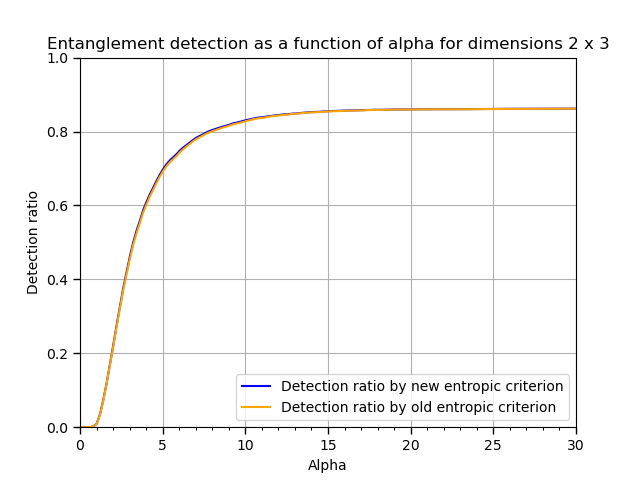
\includegraphics[width=\linewidth]{images/renyi_comparison_2_3_30_0.2.png} 
    \caption{Entanglement detection ratios as a function of $\alpha$ for dimensions 2 $\times$ 3.} 
    \label{fig:renyi_2x3} 
    \vspace{2ex}
  \end{subfigure}%% 
  \begin{subfigure}[b]{0.5\linewidth}
    \centering
    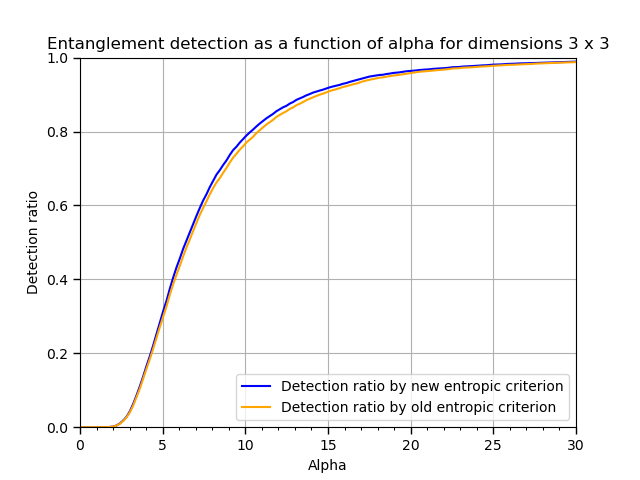
\includegraphics[width=\linewidth]{images/renyi_comparison_3_3_30_0.2.png} 
    \caption{Entanglement detection ratios as a function of $\alpha$ for dimensions 3 $\times$ 3.} 
    \label{fig:renyi_3x3} 
    \vspace{2ex}
  \end{subfigure} 
  \begin{subfigure}[b]{0.5\linewidth}
    \centering
    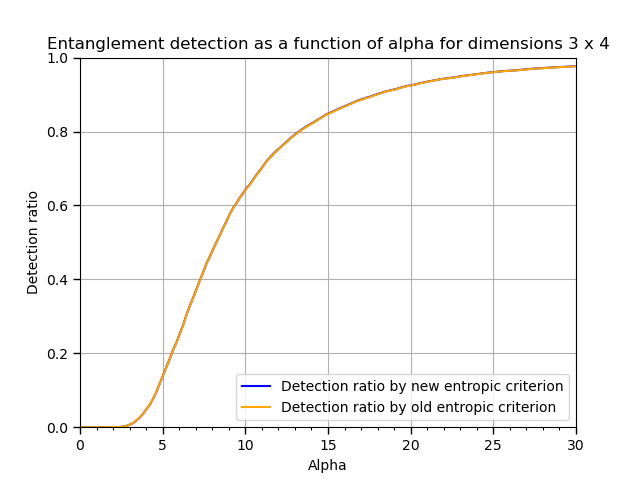
\includegraphics[width=\linewidth]{images/renyi_comparison_3_4_30_0.2.png} 
    \caption{Entanglement detection ratios as a function of $\alpha$ for dimensions 3 $\times$ 4.} 
    \label{fig:renyi_3x4} 
  \end{subfigure}%%
  \begin{subfigure}[b]{0.5\linewidth}
    \centering
    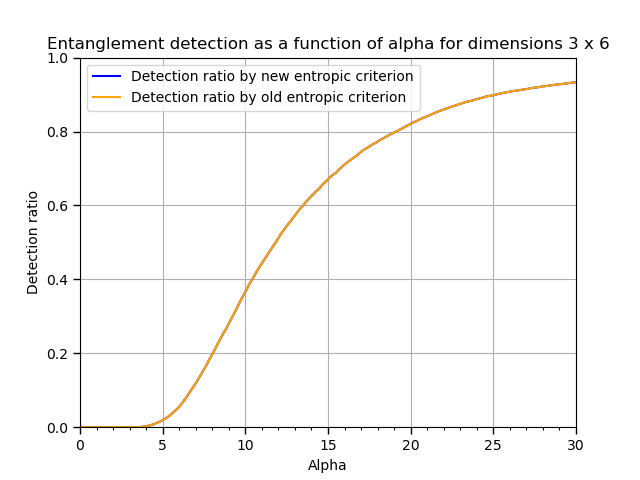
\includegraphics[width=\linewidth]{images/renyi_comparison_3_6_30_0.2.png} 
    \caption{Entanglement detection ratios as a function of $\alpha$ for dimensions 3 $\times$ 6.} 
    \label{fig:renyi_3x6} 
  \end{subfigure} 
  \caption{Comparison of the entanglement criteria for various subsystem dimensions.}
  \label{fig:renyi_comparison} 
\end{figure}

Interestingly, the Rényi simulation shows that there does seem to be an optimum $\alpha$. Moreover, it seems to be dimension-dependent (see shift between Figures \ref{fig:renyi_2x3} and \ref{fig:renyi_3x3}), with a clear optimum in dimension 3 $\times$ 3. Perhaps this hints at some deeper connection between Rényi entropy and majorization, but this research avenue was not explored further. It is also interesting to note that the improved criterion does not seem to show significant improvements according to the simulation. This might be because of a non-uniform density of quantum states in the $\Delta_{d-1}$ simplex, which might lead to a significant number of random density matrices being drawn close to the bottom of the lattice where both criteria can tell entanglement. Perhaps, instead, this might be due to reduced states of a density matrix not tending to be too imcomparable from each other, and thus being close to their meet\footnote{This is partly explained in Section \ref{sec:p_monotonicity} with Corollary \ref{cor:incomparability_separability}.}. This final idea leads nicely into the second part of this chapter, where we define and study new objects quantifying the incomparability between probability vectors.



\section{Entropic distance approach}

\subsection{Resource-theoretic intuition}

The approach that was taken was to take inspiration from resource theories to define incomparability monotones. What is often done in resource theories is to define a monotone as being the minimum distance from the studied state to the set of free states. For instance, the entanglement monotone $H(\lambda_\psi)$ is such a monotone. Consider the entropic distance (cf. section \ref{sec:entropic_distances}) $d(\lambda_\psi, \lambda_{\text{free}})$. We know that all minimally entangled states have $\lambda_\text{free} = \overline{1}_d = (1, 0, \dots, 0)$ (they are separable), and so the entropic distance reduces to

\begin{align}
    d(\lambda_\psi, \lambda_\text{free}) &= H(\lambda_\psi) + H(\lambda_\text{free}) - 2 H(\lambda_\psi \vee \lambda_\text{free})\\
                                      &= H(\lambda_\psi),
\end{align}

\noindent where $H(\lambda_\text{free}) = 0$ (the certain distribution has no entropy) and $\lambda_\psi \vee \lambda_\text{free} = \lambda_\text{free}$ because the certain distribution is the bottom of the lattice. In this particular case, there is no need to take the minimum over all free states because they all have the same Schmidt vector, but in other resource theories or using other notions of distance between quantum states, they might not all be at the same distance from the state $\lambda_\psi$.

\subsection{Expected properties}

There are some key differences to usual resource monotones when quantifying incomparability. The first major difference is that a vector can only be incomparable to another vector (a vector is not incomparable in and of itself). As such, treating incomparability as a resource is a bit strange because it would characterize some form of collective property of a pair of states, rather than an intrinsic property of individual states which most resource theories do. In the following, we will call $p$ the \textit{probe state}, and $q$ the \textit{reference state} that $p$ is compared to. Of course, nothing prevents us from reversing the roles of $p$ and $q$ to study the other half of the collective property. 

Let $E$ be some incomparability function. To emphasize the asymmetrical role of $p$ and $q$, we propose the notation $E(p \parallel q)$, which is inspired by the notation for the \textit{relative entropy} (also known as Kullback-Leibler divergence, cf. appendix \ref{app:shannon_compositions}) between 2 probability distributions, which is also asymmetric \cite[p. 19]{cover_elements_2006}. A good measure of incomparability $E$ between $p$ and $q$ should be 0 when $p \sim q$ and greater than 0 only when $p \nsim q$. That is,

\begin{equation} % peut etre moyen d'expliquer ceci un peu mieux en disant que 0 sinon ?
    E(p \parallel q) \neq 0 \iff p \in \mathcal{T}_\emptyset(q). \label{eq:ideal_incomparability}
\end{equation}

Unfortunately, the second difference with usual resource monotones is that the set of comparable vectors to $q$ is not convex. Figure \ref{fig:convex_mixture_incomp} illustrates why this is the case: a convex mixture of a vector from $\mathcal{T}_+(q)$ and $\mathcal{T}_-(q)$ could land in $\mathcal{T}_\emptyset(q)$. % ?? check le souci enft je vois pas exactement ce qui va pas
This problem unfortunately prevents us from achieving a monotone obeying equation (\ref{eq:ideal_incomparability}), at least directly. However, we can define two separate notions of incomparability, one as the minimal distance to the future cone of $q$ and the other as the minimal distance to the past cone of $q$.

\begin{figure}[h!]
    \centering
    \begin{tikzpicture}[scale=0.9]
        % draw cone of q
        \coordinate (A) at (-2,3);
        \coordinate (B) at (2, -3);
        \draw [name path=A--B] (A) -- (B);
        \coordinate (C) at (-2,-3);
        \coordinate (D) at (2,3);
        \draw [name path=C--D] (C) -- (D);
        \path [name intersections={of=A--B and C--D,by=E}];
        \node [fill=black,inner sep=1pt,label=0:$q$] at (E) {};
        % define q^- and q^+
        \coordinate (F) at (1, 2);
        \coordinate (G) at (1, -2);
        \node [fill=black,inner sep=1pt,label=90:$q^-$] at (F) {};
        \node [fill=black,inner sep=1pt,label=270:$q^+$] at (G) {};
        % draw their convex mixtures
        \draw[dotted] [name path=F--G, color=gray] (F) -- (G);
        % fill draw the future cone of p + notation
        \fill[fill=red, opacity=0.2] (C) -- (E) -- (B) -- cycle;
        \node [inner sep=0pt, label=-90:$\mathcal{T}_+ (q)$] at (0, -2) {};
        % fill draw the past cone of p + notation
        \fill[fill=blue, opacity=0.2] (A) -- (E) -- (D) -- cycle;
        \node [inner sep=0pt, label=90:$\mathcal{T}_- (q)$] at (0, 2) {};
        \node [inner sep=0pt, label=180:$\mathcal{T}_\emptyset (q)$] at (-1.5, 0) {};

    
    \end{tikzpicture}
    \caption{Depiction of the set $\mathcal{T}_+(q) \cup \mathcal{T}_-(q)$ not being convex, as there exists elements $q^+, q^-$ such that the chord joining them is not entirely contained in the set.}
    \label{fig:convex_mixture_incomp}
\end{figure}

\subsection{Future incomparability function}

Considering the previous discussion, there are 2 notions of incomparability we can define. The first will be called the notion of \textit{future incomparability}. Essentially, it is simply going to characterize how far $p$ is from the future cone of $q$. We propose the following definition for a future incomaparability function $E^+(p \parallel q)$, illustrated by figure \ref{fig:future_closest_intuition} directly on the lattice.

\begin{figure}[h!]
    \centering
    \begin{tikzpicture}[scale=0.9]
        % draw cone of q
        \coordinate (A) at (-2,3);
        \coordinate (B) at (2, -3);
        \draw [name path=A--B] (A) -- (B);
        \coordinate (C) at (-2,-3);
        \coordinate (D) at (2,3);
        \draw [name path=C--D] (C) -- (D);
        \path [name intersections={of=A--B and C--D,by=E}];
        \node [fill=black,inner sep=1pt,label=0:$q$] at (E) {};
        % ghost draw cone of p
        \coordinate (F) at (0.666,3);
        \coordinate (G) at (-3.333, -3);
        \draw [name path=F--G, draw=none] (F) -- (G);
        \coordinate (H) at (-0.666,-3);
        \coordinate (I) at (-4.666,3);
        \draw [name path=H--I, draw=none] (H) -- (I);
        \path [name intersections={of=F--G and H--I,by=J}];
        \node [fill=black,inner sep=1pt,label=180:$p$] at (J) {};
        \path [name intersections={of=F--G and A--B,by=K}];
        \path [name intersections={of=H--I and C--D,by=L}];
        %\node [fill=black,inner sep=2pt,label=180:closest past state?] at (K) {};
        \node [fill=black,inner sep=1.5pt,label=180:closest future state] at (L) {};
        %\draw[dotted] [name path=J--K, color=gray] (J) -- (K);
        \draw[dotted] [name path=J--L, color=gray] (J) -- (L) node[midway, above, sloped] {$E^+(p \parallel q)$};
        % fill draw the future cone of p + notation
        \fill[fill=red, opacity=0.2] (C) -- (E) -- (B) -- cycle;
        \node [inner sep=0pt, label=-90:$\mathcal{T}_+ (q)$] at (0, -2) {};
        % fill draw the past cone of p + notation
        %\fill[fill=blue, opacity=0.2] (A) -- (E) -- (D) -- cycle;
        %\node [inner sep=0pt, label=90:$\mathcal{T}_- (q)$] at (0, 2) {};
        % fill draw the incomparable region of p mais pas hyper clair
        %\filldraw[draw=black, fill=gray, opacity=0.2] (A) -- (E) -- (C) -- cycle;
        %\filldraw[draw=black, fill=gray, opacity=0.2] (D) -- (E) -- (B) -- cycle;
        %\node [inner sep=0pt, label=0:$\mathcal{T}_\emptyset (q)$] at (1.5, 0) {};
    
    \end{tikzpicture}
    \caption{Depiction of the geometrical intuition behind the closest 'free state' approach.}
    \label{fig:future_closest_intuition}
\end{figure}

\begin{definition}[Future incomparability function] \label{def:future_incomparability_monotone}
    Let $p, q \in \mathcal{P}^d$. The future incomparability $E^+(p \parallel q)$ of $p$ to $q$ is defined as
    \begin{equation}
        E^+ (p \parallel q) = \min_{s \succ q} d(p, s).
    \end{equation}
\end{definition}

\begin{remark}
    From the definition it is easy to see that $p \in \mathcal{T}_+(q) \iff E^+(p \parallel q) = 0$, because then the closest state to $p$ that also majorizes $q$ is simply $p$.
\end{remark}

Essentially, we are looking for the vector $s$ in $\mathcal{T}_+(q)$ which is closest to $p$ in terms of entropic distance. Intuitively, we would expect this vector to be $p \vee q$. Lemma \ref{lem:comp_future} gives us the tools to prove the first major result of this chapter, which essentially states that our geometric intuition is correct.

\begin{theorem}
    The future incomparability of a vector $p$ to another vector $q$ is the entropic distance from $p$ to their join. Formally,
    \begin{equation}
        E^+ (p \parallel q) = d(p, p \vee q).
    \end{equation}
\end{theorem}

Essentially, this theorem simply states that our geometric intution concerning majorization cones is correct (in this case). Let us now prove this result.

\begin{proof}
    Let us find the minimal value of $d(p, s)$ (with $s \succ q$), and let us show that it is realized for $s = p \vee q$.

    \begin{align}
        E^+(p \parallel q) &= \min_{s \succ q} d(p, s) \\
        \overset{\text{Lemma \ref{lem:comp_future}}}&{=} \min_{s \succ q} d(p, p \vee s) + d(p \vee s, s)
    \end{align}

    \noindent Let $s' = p \vee s$. The absorption law $a \vee a = a$, along with the associativity of the join operation, implies that choosing $s = s'$ (i.e. requiring that $s$ majorizes $p$) makes the second term of the sum vanish, while the first remains invariant.

    \begin{align}
        \implies E^+ (p \parallel q) &= \min_{s \succ q} d(p, p \vee s') + d(p \vee s', s') \\
        &= \min_{s \succ q} d(p, p \vee (p \vee s)) + d(p \vee (p \vee s), p \vee s) \\
        &= \min_{s \succ q} d(p, (p \vee p) \vee s) + d((p \vee p) \vee s, p \vee s)\\
        &= \min_{s \succ q} d(p, p \vee s) + d(p \vee s, p \vee s)\\
        &= \min_{s \succ q} d(p, p \vee s)
    \end{align}

    \noindent Because $s$ majorizes $q$, $s'$ majorizes $q$ too. Moreover, to be the join of $p$ with another vector, $s'$ must majorize $p$ as well.

    \begin{align}
        \implies E^+ (p \parallel q) &= \min_{s' \succ q, p} d(p, s') \\
        &= \min_{s' \succ q, p} H(p) + H(s') - 2H(p \vee s') \\
        &= \min_{s' \succ q, p} H(p) + H(s') - 2H(s') \\
        &= \min_{s' \succ q, p} H(p) - H(s').\\
    \end{align}

    \noindent The Schur-concavity of the Shannon entropy implies that the maximum value of $H(s')$ for $s' \in \{v \mid v \succ p, q\}$\footnote{This is equivalent to saying $s' \in \mathcal{T}_+(p) \cap \mathcal{T}_+(q)$.}$ \subseteq \mathcal{P}^d$ is reached for a vector $s'$ that is majorized by all other vectors in the subset. By definition, that vector is the join $p \vee q$. \qedhere
\end{proof}



\subsection{Past incomparability function}

One could attempt the same definition for a \textit{past incomparability} function of $p$ to $q$ as being the minimal distance from $p$ to the past cone of $q$, $\mathcal{T}_-(q)$. However, using the same entropic distance does not yield properties as nice as we had with the join. A simple interpretation of this would be the hyperbolic geometry induced by our entropic distance, which complicates any attempts at working with the meet. Instead, we worked with the entropic quasidistance $d'(p, q) = 2H(p \wedge q) - H(p) - H(q)$ as introduced in definition \ref{def:entropic_quasidistance}. We propose the following definition for a past incomparability function $E^-(p \parallel q)$, illustrated by figure \ref{fig:past_closest_intuition}.

\begin{figure}[h!] % rajouter les 4 distances sur la figure ?
    \centering
    \begin{tikzpicture}[scale=0.9]
        % draw cone of q
        \coordinate (A) at (-2,3);
        \coordinate (B) at (2, -3);
        \draw [name path=A--B] (A) -- (B);
        \coordinate (C) at (-2,-3);
        \coordinate (D) at (2,3);
        \draw [name path=C--D] (C) -- (D);
        \path [name intersections={of=A--B and C--D,by=E}];
        \node [fill=black,inner sep=1pt,label=0:$q$] at (E) {};
        % ghost draw cone of p
        \coordinate (F) at (0.666,3);
        \coordinate (G) at (-3.333, -3);
        \draw [name path=F--G, draw=none] (F) -- (G);
        \coordinate (H) at (-0.666,-3);
        \coordinate (I) at (-4.666,3);
        \draw [name path=H--I, draw=none] (H) -- (I);
        \path [name intersections={of=F--G and H--I,by=J}];
        \node [fill=black,inner sep=1pt,label=180:$p$] at (J) {};
        \path [name intersections={of=F--G and A--B,by=K}];
        %\path [name intersections={of=H--I and C--D,by=L}];
        \node [fill=black,inner sep=1.5pt,label=180:closest past state] at (K) {};
        %\node [fill=black,inner sep=2pt,label=180:closest future state?] at (L) {};
        \draw[dotted] [name path=J--K, color=gray] (J) -- (K) node[midway, below, sloped] {$E^-(p \parallel q)$};
        %\draw[dotted] [name path=J--L, color=gray] (J) -- (L);
        % fill draw the future cone of p + notation
        %\fill[fill=red, opacity=0.2] (C) -- (E) -- (B) -- cycle;
        %\node [inner sep=0pt, label=-90:$\mathcal{T}_+ (q)$] at (0, -2) {};
        % fill draw the past cone of p + notation
        \fill[fill=blue, opacity=0.2] (A) -- (E) -- (D) -- cycle;
        \node [inner sep=0pt, label=90:$\mathcal{T}_- (q)$] at (0, 2) {};
        % fill draw the incomparable region of p mais pas hyper clair
        %\filldraw[draw=black, fill=gray, opacity=0.2] (A) -- (E) -- (C) -- cycle;
        %\filldraw[draw=black, fill=gray, opacity=0.2] (D) -- (E) -- (B) -- cycle;
        %\node [inner sep=0pt, label=0:$\mathcal{T}_\emptyset (q)$] at (1.5, 0) {};
    
    \end{tikzpicture}
    \caption{Depiction of the geometrical intuition behind the closest 'free state' approach.}
    \label{fig:past_closest_intuition}
\end{figure}

\begin{definition}[Past incomparability function]
    Let $p, q \in \mathcal{P}^d$. The past incomparability $E^-(p \parallel q)$ of $p$ to $q$ is defined as
    \begin{equation}
        E^- (p \parallel q) = \min_{s \prec q} d'(p, s).
    \end{equation}
\end{definition}

The same interpretation can be given as the future incomparability function, though one should be careful that we are working with a quasidistance this time around, and so geometric intuitions can be deceiving.

\begin{remark}
    From the definition it is easy to see that $p \in \mathcal{T}_-(q) \iff E^-(p \parallel q) = 0$, because then the closest state to $p$ that is also majorized by $q$ is simply $p$.
\end{remark}

With this quasidistance, we fall on similar properties as we did with the future incomparability monotone. Namely, the minimal quasidistance to the past cone is reached for the meet $p \wedge q$. Before proving this, we will need the following lemma, very similar to lemma \ref{lem:comp_future} except that this time around we cannot speak of triangular inequality because of the quasidistance.

\begin{lemma} \label{lem:comp_past}
    Let $p, q \in \mathcal{P}^d$. For the entropic quasidistance $d'(p, q) = 2H(p \wedge q) - H(p) - H(q)$, we have
    \begin{equation}
        d'(p, q) = d'(p, p \wedge q) + d'(p \wedge q, q).
    \end{equation}
\end{lemma}

\begin{proof}
    \begin{align}
        d'(p, p \wedge q) + d'(p \wedge q, q) &= 2H(p \wedge (p \wedge q)) - H(p) - H(p \wedge q) + 2H((p \wedge q) \wedge q) \nonumber\\
        &\quad \quad - H(p \wedge q) - H(q)\\
        &= 2H(p \wedge q) - H(p \wedge q) - H(p) + 2H(p \wedge q) - H(p \wedge q)\nonumber\\
        &\quad \quad - H(q) \\
        &= 2H(p \wedge q) - H(p) - H(q) \\
        &= d'(p, q). \qedhere
    \end{align} 
\end{proof}

We are now ready to prove the main result of this section, which again states that our geometric intuition is correct (though this time the interpretation is murkier given the quasidistance).

\begin{theorem}
    The past incomparability of a vector $p$ to another vector $q$ is the entropic distance\footnote{While the definition made no mention of the rigorous entropic distance $d$, this theorem brings us back to the actual distance.} from $p$ to their meet. Formally,
    \begin{equation}
        E^- (p \parallel q) = d(p, p \wedge q).
    \end{equation}
\end{theorem}

\begin{proof}
    Let us find the minimal value of $d'(p, s)$ (with $s \prec q$), and let us show it is realized for $s = p \wedge q$.
    \begin{align}
        E^- (p \parallel q) &= \min_{s \prec q} d'(p, s) \\
        \overset{\text{Lemma \ref{lem:comp_past}}}&{=} \min_{s \prec q} d'(p, p \wedge s) + d'(p \wedge s, s) \\ 
        &\implies \min_{s \prec q} d'(p, s) \geq \min_{s \prec q} d'(p, p \wedge s) \label{eq:1}
    \end{align}

    \noindent Let $s' = p \wedge s$. Because $s$ is majorized by $q$, $s'$ is majorized by $q$ as well. Moreover, to be the meet of $p$ with another vector, $s'$ must be majorized by $p$ as well.

    \begin{align}
        \implies \min_{s \prec q} d'(p, p \wedge s) &= \min_{s' \prec q, p} d'(p, s')\\
        &= \min_{s' \prec q, p} 2H(p \wedge s') - H(p) - H(s')\\
        &= \min_{s' \prec q, p} H(s') - H(p).
    \end{align}

    \noindent The Schur-concavity of the Shannon entropy implies that the minimum value of $H(s')$ for  $s' \in \{v \mid v \prec p, q\}$\footnote{This is equivalent to saying $s' \in \mathcal{T}_-(p) \cap \mathcal{T}_-(q)$.}$ \subseteq \mathcal{P}^d$ is reached for a vector $s'$ that majorizes all other vectors in the subset. By definition, that vector is the meet $p \wedge q$, and so $\min_{s' \prec q, p} H(s') - H(p) = H(p \wedge q) - H(p)$. The vector $p \wedge q$ is also part of the original subset $\{v \mid v \prec q\}$, and so plugging $s = p \wedge q$ into (\ref{eq:1}) shows that the LHS realizes the value $H(p \wedge q) - H(p)$ as well, and the 2 minima must therefore be equal. Moreover, at the final line we have $H(s') - H(p) = d'(s', p) = d(s', p)$, because the two distance notions are equal when vectors are comparable. \qedhere
\end{proof}



\section{Properties}

For this section, we will denote bistochastic matrices of dimension $d\times d$ by the letter $D$. Recall that an equivalent definition of majorization is $p \prec q \iff \exists D \: | \: q = Dp$ (cf. section \ref{sec:bistochastic}). Now that we have defined our two incomparability functions and shown that they are equal to the (quasi)distance to the meet or join, let us show that they are monotones under a bistochastic degradation. Conversely, if they are increasing (resp. decreasing) monotones under a bistochastic degradation, they are a decreasing (resp. increasing) monotone under a LOCC degradation in the quantum picture. However, we are working with 2 states, and so we can study degradations of $p$ and of $q$ separately.



\subsection{Monotonicity under bistochastic degradation of the probe} \label{sec:p_monotonicity}

Let us start with studying the future incomparability function. If we can show that $E^+(Dp \parallel q)$ is greater than $E^+(p \parallel q)$ for any bistochastic matrix $D$ (implying $Dp \in \mathcal{T}_-(p)$), then we can promote our future incomparability function $E^+$ to an increasing monotone under bistochastic degradation of $p$, or alternatively to a decreasing monotone under LOCC degradation. Figure \ref{fig:future_p_monotonicity} shows why we geometrically expect this to be the case. The representation seems to indicate that the states with the lowest distance to $\mathcal{T}_+(q)$ are on the edge facing towards $q$. All of the states on the edge visually have the same distance to the cone, like $p'$. But remembering the hyperbolic metric induced by the entropic distance (cf. section \ref{sec:entropic_distances}), we deduce that $d(p', p' \vee q) \geq d(p, p \vee q)$ for any $p'$ on that edge.

\begin{figure}[h!] % rajouter les 4 distances sur la figure ?
    \centering
    \begin{tikzpicture}[scale=0.9]
        % draw cone of q
        \coordinate (A) at (0, 3);
        \coordinate (B) at (-2,0);
        \coordinate (C) at (2, 0);
        \draw [name path=A--B] (A) -- (B);
        \draw [name path=A--C] (A) -- (C);
        \node [fill=black,inner sep=1pt,label=0:$q$] at (A) {};
        % drawfill future cone of q
        \fill[fill=red, opacity=0.2] (A) -- (B) -- (C) -- cycle;
        \node [inner sep=0pt, label=-90:$\mathcal{T}_+ (q)$] at (0, 1.5) {};
        % draw cone of p
        \coordinate (D) at (-2, 1.5);
        \coordinate (E) at (-4, 4.5);
        \coordinate (F) at (0, 4.5);
        \draw[dotted] [name path=D--E, color=red] (D) -- (E);
        \draw[dotted] [name path=D--F, color=red] (D) -- (F);
        \node [fill=black,inner sep=1pt,label=225:$p$] at (D) {};
        % draw bottom right leg for p
        \coordinate (K) at (-1, 0);
        \draw[draw=none] [name path=D--K] (D) -- (K);
        \path [name intersections={of=D--K and A--B, by=L}];
        \draw[dotted] [name path=D--L, color=gray] (D) -- (L);
        % add p' and p''
        \coordinate (P') at (-1, 3);
        \coordinate (P'') at (-2.5, 3.5);
        \node [fill=black,inner sep=1pt,label=90:$p'$] at (P') {};
        \node [fill=black,inner sep=1pt,label=145:$p''$] at (P'') {};
        % ghost draw bottom right cone leg for p' and p''
        \coordinate (G) at (1, 0);
        \coordinate (H) at (-0.16666, 0);
        \draw[draw=none] [name path=P'--G] (P') -- (G);
        \draw[draw=none] [name path=P''--H] (P'') -- (H);
        \path [name intersections={of=P'--G and A--B, by=I}];
        \path [name intersections={of=P''--H and A--B, by=J}];
        \draw[dotted] [name path=P'--I, color=gray] (P') -- (I);
        \draw[dotted] [name path=P''--J, color=gray] (P'') -- (J);

    \end{tikzpicture}
    \caption{Depiction of the expected monotonicity in $p$ of $E^+$. The dotted red half-cone contains all possible bistochastic degradations of $p$.}
    \label{fig:future_p_monotonicity}
\end{figure}

\noindent In order to rigorously prove monotonicity, we will first need the following lemma (cf. figure \ref{fig:hyperbolic_geometry}).

\begin{lemma} \label{lem:incomparable_diamond}
    In any incomparable diamond $p, q, p \wedge q, p \vee q$ we have $d(p, p \vee q) \leq d(q, p \wedge q)$.
\end{lemma}

\begin{proof}
    Let $p, q \in \mathcal{P}^d$. We have
    \begin{align}
        d(p, p \vee q) &= H(p) + H(p \vee q) - 2H(p \vee (p \vee q))\\
        &= H(p) - H(p \vee q)\\
        &= H(p) + H(p \wedge q) - H(p \wedge q) - H(p \vee q)\\
        \overset{\text{supermod}}&{\leq} H(p \wedge q) - H(q)\\
        &= d(q, p \wedge q). \qedhere
    \end{align} 
\end{proof}

This lemma is essentially just an equivalent way of stating supermodularity. We are now ready to prove the main theorem of this section.

\begin{theorem} \label{th:monotone_future_p}
    There exists no bistochastic matrix $D$ such that $E^+ (Dp \parallel q) < E^+ (p \parallel q)$.
\end{theorem}

This theorem essentially states that $E^+$ is an increasing monotone under bistochastic degradation of $p$. This proof is perhaps the trickiest of the chapter, so figure \ref{fig:future_p_monotonicity_construction} illustrates the different vectors of the construction on the lattice to help with comprehension.

\begin{proof}
    Let us show that the minimal value of $E^+ (p' \parallel q)$ (with $p' \prec p$) is realized for $p' = p$. Let $p'$ be a vector majorized by $p$, i.e. there exists a bistochastic matrix $D$ such that $p' = Dp$. Let $q'(p') = p' \vee q$, and let $p''(p') = p \wedge q'$ which are both functions of the variable to minimize over, $p'$. To avoid cluttering the expressions, we will simply write $p''$ and $q'$, but one should keep in mind that they are indeed functions of $p'$. By hypothesis and by definition of $q'$, $p'$ is majorized by both $p$ and $q'$, which is equivalent to $p'$ being majorized by $p \wedge q'$. We have

    \begin{equation}
         d(p'', q') = H(p \wedge q') - H(q') \leq H(p') - H(q') = d(p', q'), \label{eq:construction}
    \end{equation} 

    \noindent which can be used for the following development

    \begin{align}
        \min_{p' \prec p} E^+ (p' \parallel q) &= \min_{p' \prec p} d(p', p' \vee q)\\
        &= \min_{p' \prec p} d(p', q')\\
        \overset{\text{(\ref{eq:construction})}}&{=} \min_{p' \prec p} d(p'', q')\\
        &= \min_{p' \prec p} d(p \wedge q', q')\\
        \overset{\text{Lemma \ref{lem:incomparable_diamond}}}&{\geq} \min_{p' \prec p} d(p, p \vee q')\\
        &= \min_{p' \prec p} d(p, p \vee (p' \vee q))\\
        &= \min_{p' \prec p} d(p, (p \vee p') \vee q)\\
        &= d(p, p \vee q)\\
        &= E^+ (p \parallel q),
    \end{align}
    \noindent and so the minimal value of $E^+ (Dp \parallel q)$ is reached for the identity degradation which leaves $p$ invariant. \qedhere
\end{proof}

\begin{figure}[h!] % rajouter les 4 distances sur la figure ?
    \centering
    \begin{tikzpicture}[scale=0.9]
        % draw cone of q
        \coordinate (Q) at (0, 3);
        \coordinate (B) at (-2,0);
        \coordinate (C) at (2, 0);
        \draw [name path=Q--B] (Q) -- (B);
        \draw [name path=Q--C] (Q) -- (C);
        \node [fill=black,inner sep=1pt,label=0:$q$] at (Q) {};
        % drawfill future cone of q
        \fill[fill=red, opacity=0.2] (Q) -- (B) -- (C) -- cycle;
        \node [inner sep=0pt, label=-90:$\mathcal{T}_+ (q)$] at (0, 1.5) {};
        % draw cone of p
        \coordinate (P) at (-2, 1.5);
        \coordinate (E) at (-4, 4.5);
        \coordinate (F) at (0, 4.5);
        \draw[dotted] [name path=P--E, color=red] (P) -- (E);
        \draw[dotted] [name path=P--F, color=red] (P) -- (F);
        \node [fill=black,inner sep=1pt,label=225:$p$] at (P) {};
        % draw bottom right leg for p
        \coordinate (K) at (-1, 0);
        \draw[draw=none] [name path=P--K] (P) -- (K);
        \path [name intersections={of=P--K and Q--B, by=L}];
        \draw[dotted] [name path=P--L, color=gray] (P) -- (L);
        % add p'
        \coordinate (P') at (-2, 4);
        \node [fill=black,inner sep=1pt,label=145:$p'$] at (P') {};
        % ghost draw bottom right cone leg for p'
        \coordinate (H) at (0.66666, 0);
        \draw[draw=none] [name path=P'--H] (P') -- (H);
        \path [name intersections={of=P'--H and Q--B, by=Q'}];
        \draw[dotted] [name path=P'--Q', color=gray] (P') -- (Q');
        % add q'
        \node [fill=black,inner sep=1pt,label=0:$q'$] at (Q') {};
        % add p''
        \path [name intersections={of=P'--H and P--F, by=P''}];
        \node [fill=black,inner sep=1pt,label=180:$p''$] at (P'') {};
        

    \end{tikzpicture}
    \caption{Depiction of the lattice construction for the proof of theorem \ref{th:monotone_future_p}. Essentially, the purpose of $q'$ is only to define $p''$ from $q'$, which is guaranteed to be on the edge closest to $q$ where the (visually) closest points to $\mathcal{T}_+(q)$ lie no matter the choice of $p'$.}
    \label{fig:future_p_monotonicity_construction}
\end{figure}
 
This theorem is quite satisfying in the sense that it seems to indicate that our geometric intuitions on the lattice are valid. Moreover, we can now promote the future incomparability function to a future incomparability \textit{monotone}. Theorem \ref{th:monotone_future_p} has a few corollaries.

\begin{corollary} \label{cor:incomparability_LOCC}
    Let $\ket{\psi}$ and $\ket{\phi}$ be two pure quantum states, and let $\lambda_\psi$ and $\lambda_\phi$ be the associated Schmidt vectors. If $\ket{\psi} \overset{\text{LOCC}}{\longrightarrow} \ket{\phi}$ with probability 1, then $E^+ (\lambda_\psi \parallel \lambda_\alpha) \geq E^+ (\lambda_\phi \parallel \lambda_\alpha)$ with $\lambda_\alpha$ some probability vector.
\end{corollary}

\begin{corollary} \label{cor:incomparability_separability}
    Let $\rho_{AB}$ be a bipartite quantum state, and let $\rho_A$ and $\rho_B$ be the reduced states. Let $\lambda_{AB}, \lambda_A$ and $\lambda_B$ be the vectors of eigenvalues of their density matrices. Then, if $\rho_{AB}$ is separable, $E^+ (\lambda_{AB} \parallel \lambda_B) \geq E^+ (\lambda_A \parallel \lambda_B)$ and $E^+ (\lambda_{AB} \parallel \lambda_A) \geq E^+ (\lambda_B \parallel \lambda_A)$.
\end{corollary}

These corollaries, while not very useful per se, still hold some interpretational value, because they show that in the sense of our future incomparability monotone, some states must be more incomparable than others relatively to some set states. Corollary \ref{cor:incomparability_LOCC}, while involving some nondescript Schmidt vector $\lambda_\alpha$, essentially states it is not possible to create a state that is more incomparable to $\lambda_\alpha$ through LOCC than the original state $\lambda_\psi$. Corollary \ref{cor:incomparability_separability} is perhaps more interesting, and states that if a joint state is separable, then the joint state is more incomparable to each of the reduced states than the reduced states are to each other. The converse might partly explain the discussion at the end of chapter \ref{chap:criteria}: if a state is strongly entangled, then it is more incomparable to each of the reduced states than they are between each other. Therefore, such states tend to not have particularly incomparable $\lambda^A$ and $\lambda^B$, which also means that their meet is fairly close, and so the improved criterion involving the meet is not a significant improvement, especially considering that $\lambda^{AB}$ cannot be too close to them.

One would hope that the analogue of theorem \ref{th:monotone_future_p} would hold for the measure of past incomparability $E^-$, however it does not. The following counterexample shows that a bistochastic matrix $D$ such that $E^- (Dp \parallel q) < E^- (p \parallel q)$ can exist, but also that a bistochastic matrix $D'$ such that $E^- (D'p \parallel q) > E^- (p \parallel q)$ can exist too. Let $q = (0.6, 0.4)$, $p = (0.7, 0.29, 0.01)$, $p' = p \wedge q$ and $p'' = (0.7, 0.15, 0.15)$. One can verify that $p$ majorizes both $p'$ and $p''$, yet $E^- (p \parallel q) = 0.0939$ bits, $E^- (p' \parallel q) = 0$ bits and $E^- (p'' \parallel q) = 0.171$ bits. With figure FAIRE FIGURE it is not too hard to see that this is because the hyperbolic geometry makes distance in the wrong way in this case: sticking to the right edge for $p'$ makes $E^-$ increase, whereas with $p''$ one can go straight towards the past cone of $q$, making $E^-$ decrease, and so there is no monotonicity.



\subsection{Monotonicity under bistochastic degradation of the reference} \label{sec:q_monotonicity}

Let us now turn our attention to bistochastic degradations of $q$, and attempt to promote our incomparability functions to monotones. Figure \ref{fig:future_q_monotonicity} shows the monotonicity relations we expect. The proofs of these properties are simpler than for probe degradation, and can be found in appendix \ref{app:q_monotonicity}. Starting with the future incomparability function, if we can show that $E^+(p \parallel Dq) < E^+(p \parallel q)$ for any bistochastic matrix $D$, then $E^+$ would be a decreasing monotone, like we expect.

\begin{figure}[h!] % rajouter les 4 distances sur la figure ?
    \centering
    \begin{minipage}{.48\textwidth}
        \centering
        \begin{tikzpicture}[scale=0.9]
            % draw cone of q
            \coordinate (Q) at (0, 3);
            \coordinate (B) at (-2,0);
            \coordinate (C) at (2, 0);
            \draw[dotted] [name path=Q--B, color=gray] (Q) -- (B);
            \draw[dotted] [name path=Q--C, color=gray] (Q) -- (C);
            \node [fill=black,inner sep=1pt,label=0:$q$] at (Q) {};
            \coordinate (E) at (-2, 6);
            \coordinate (F) at (2, 6);
            \draw[dotted] [name path=Q--E, color=red] (Q) -- (E);
            \draw[dotted] [name path=Q--F, color=red] (Q) -- (F);
            % draw cone of p
            \coordinate (P) at (-3, 3);
            \node [fill=black,inner sep=1pt,label=0:$p$] at (P) {};
            \coordinate (D) at (-1, 0);
            \draw[draw=none] [name path=P--D] (P) -- (D);
            % add q' and q''
            \coordinate (Q') at (1, 4.5);
            \coordinate (Q'') at (0, 4.5);
            \node [fill=black,inner sep=1pt,label=0:$q'$] at (Q') {};
            \node [fill=black,inner sep=1pt,label=70:$q''$] at (Q'') {};
            % draw bottom left legs of q' and q''
            %\coordinate (Z') at (-3, 0);
            \coordinate (Z'') at (-3, 0);
            %\draw[dotted] [name path=Q'--Z', color=gray] (Q') -- (Z');
            \draw[dotted] [name path=Q''--Z'', color=gray] (Q'') -- (Z'');
            % draw until intersection with initial q cone
            \path [name intersections={of=P--D and Q--B, by=I}];
            \draw[dotted] [name path=P--I, color=gray] (P) -- (I);
            

        \end{tikzpicture}
        \caption{Depiction of the expected monotonicity in $q$ of $E^+$. The dotted red half-cone contains all possible bistochastic degradations of $q$. Visually, $p$ has highest $E^+$ relative to states on the furthest edge from $p$, like $q'$, and all other choices decrease $E^+$, like $q''$. The cones of $q, q'$ and $q''$ have not been fully drawn and shaded to avoid visual cluttering.}
        \label{fig:future_q_monotonicity}
    \end{minipage}
    \hfill
    \begin{minipage}{.48\textwidth}
        \centering
        \begin{tikzpicture}[scale=0.9]
            % draw cone of q
            \coordinate (Q) at (0, 3);
            \coordinate (B) at (-1, 1.5);
            \coordinate (C) at (1, 1.5);
            \draw[draw=none] [name path=Q--B, color=gray] (Q) -- (B);
            \draw[draw=none] [name path=Q--C, color=gray] (Q) -- (C);
            \node [fill=black,inner sep=1pt,label=0:$q$] at (Q) {};
            \coordinate (E) at (-3, 7.5);
            \coordinate (F) at (3, 7.5);
            \draw[dotted] [name path=Q--E, color=red] (Q) -- (E);
            \draw[dotted] [name path=Q--F, color=red] (Q) -- (F);
            % draw cone of p
            \coordinate (P) at (-3, 3);
            \node [fill=black,inner sep=1pt,label=0:$p$] at (P) {};
            \coordinate (D) at (0, 7.5);
            \draw[draw=none] [name path=P--D] (P) -- (D);
            % add q' and q''
            \coordinate (Q') at (-1, 4.5);
            \coordinate (Q'') at (0, 4.5);
            \node [fill=black,inner sep=1pt,label=210:$q'$] at (Q') {};
            \node [fill=black,inner sep=1pt,label=70:$q''$] at (Q'') {};
            % draw bottom left legs of q' and q''
            %\coordinate (Z') at (-3, 0);
            \coordinate (Z'') at (-2, 7.5);
            %\draw[dotted] [name path=Q'--Z', color=gray] (Q') -- (Z');
            \draw[dotted] [name path=Q''--Z'', color=gray] (Q'') -- (Z'');
            % draw until intersection with initial q cone
            \path [name intersections={of=P--D and Q''--Z'', by=I}];
            \draw[dotted] [name path=P--I, color=gray] (P) -- (I);
            

        \end{tikzpicture}
        \caption{Depiction of the expected monotonicity in $q$ of $E^-$. The dotted red half-cone contains all possible bistochastic degradations of $q$. Visually, $p$ has lowest $E^-$ relative to states on the closest edge to $p$, like $q'$, and all other choices increase $E^-$, like $q''$. The cones of $q, q'$ and $q''$ have not been fully drawn and shaded to avoid visual cluttering.}
        \label{fig:past_q_monotonicity}
    \end{minipage}
\end{figure}

\begin{theorem} \label{th:monotone_future_q}
    There exists no bistochastic matrix $D$ such that $E^+ (p \parallel Dq) > E^+ (p \parallel q)$.
\end{theorem}

Let us turn our attention to $E^-$. This time around, the expected property for $E^-$ does hold, and we do have monotonicity in $q$. If we can show that $E^-(p \parallel Dq) > E^+(p \parallel q)$ for any bistochastic matrix $D$, then $E^-$ would be an increasing monotone, like we expect.

\begin{theorem} \label{th:monotone_past_q}
    There exists no bistochastic matrix $D$ such that $E^- (p \parallel Dq) < E^- (p \parallel q)$.
\end{theorem}

To conclude this section, we will simply note that theorems \ref{th:monotone_future_q} and \ref{th:monotone_past_q} have similar corollaries to those of theorem \ref{th:monotone_future_p}.

\begin{remark}
    While theorems \ref{th:monotone_future_q} and \ref{th:monotone_past_q} imply that the maximal value of $E^+$ and the minimal value of $E^-$ are reached for the identity degradation of $q$, other degradations can also lead to the same value. This is made clearer by comparing the figure for $p$ monotonicity \ref{fig:future_p_monotonicity} and the figures for $q$ monotonicitity \ref{fig:future_q_monotonicity}, \ref{fig:past_q_monotonicity}, and we can see that the situation in $p$ and $q$ is a bit different. In $p$, the minimal value is reached \textit{only} for $Dp = p$, whereas in $q$ there are other states in $\mathcal{T}_-(q)$ that lead to the same value of the incomparability montone. 
\end{remark}



\subsection{Compositions}

Now that we have these monotones and have proved some monotonicity properties, we could attempt to build compositions of the two that would have some nice properties. We propose the following definitions.

\begin{definition}[Distance-like incomparability function] \label{def:distance-like_function}
    Let $p, q \in \mathcal{P}^d$. The distance-like incomparability function $F$ is defined as 
    \begin{equation}
        F(p \parallel q) = E^+(p \parallel q) - E^-(p \parallel q).
    \end{equation}
\end{definition}

\begin{definition}[Area-like incomparability function] \label{def:area-like_function}
    Let $p, q \in \mathcal{P}^d$. The area-like incomparability function $G$ is defined as 
    \begin{equation}
        G(p \parallel q) = E^+(p \parallel q) E^-(p \parallel q).
    \end{equation}
\end{definition}

Both of these definitions have interesting properties that might be desirable depending on different use cases. For $F$, a nice property is that theorems \ref{th:monotone_future_q} and \ref{th:monotone_past_q} guarantee that $F$ is a decreasing monotone under bistochastic degradation of $q$. However, $F$ is not necessarily positive. It is unknown whether it is a monotone under bistochastic degradation of $p$.

For $G$, the advantage is that it is positive, and it does satisfy equation (\ref{eq:ideal_incomparability}), because $E^+(p \parallel q) = 0 \iff p \in \mathcal{T}_+(q)$ and $E^-(p \parallel q) = 0 \iff p \in \mathcal{T}_-(q)$. The only region where $G(p \parallel q) \neq 0$ is $\mathcal{T}_\emptyset(q)$, which is a very nice property for a measure of incomparability. However, $G$ loses the monotonicity under bistochastic degradation of $q$. It is unknown whether it is a monotone under bistochastic degradation of $p$.

\section{Discussion}

We will voluntarily keep the discussion in this section short because a better interpretation of $E^+$ and $E^-$ will be made possible with the properties of Shannon entropy we uncover in chapter \ref{chap:volume}. We also postpone discussing applications of those 2 monotones to chapter \ref{chap:volume}. The properties of the distance-like and area-like functions $F$ and $G$ could also be interesting to study, but another direction was chosen. Of the two, $G$ seems like the more promising candidate for a measure of incomparability between two vectors.

While we did take inspiration from a resource-theoretic approach, we have not defined a full resource theory. Indeed, although we have identified free states as being the future-comparable or past-comparable states of $q$, it is not clear what the free operations of the theory might be. Perhaps some more general notion of operation should be defined which would act on both $p$ and $q$, and where $p$ ending in a reachable region for $q$ would make it free because it is already reachable from $q$. This (potential) new type of relative resource theory might be interesting in considering the intrinsic value of having a diverse set of states: if $p \nsim q$, then $p$ can reach some states that $q$ can't (e.g. in a LOCC context). In this sense, incomparability seems like it enables \textit{diversity} in reachable states.

Therefore, incomparability seems like a desirable property, and it is this idea that was explored further. More precisely, now that we have quantified the incomparability between a probe state and a reference state, the question that ended up being interesting to ask was how can we generalize this notion of incomparability to a \textit{set of reference states}?